\chapter{地面效应下的执行器控制效益离线辨识}
涵道式无人机凭借其垂直起降能力、结构紧凑性和高气动效率，在狭小空间作业、低空物流及城市空中交通等场景中展现出独特的应用潜力。然而，当无人机在起降、低空悬停或近地飞行时，地面效应对其气动特性产生显著影响。涵道风扇的推力特性与控制舵面的操纵效率均随离地高度发生剧烈变化，若在控制器设计中忽略这一影响，将导致模型失配、控制精度下降，甚至引发飞行失稳。

地面效应下的涵道风扇流动机理极为复杂：高速旋转的螺旋桨将气流加速并经由涵道向下排出，当无人机接近地面时，该射流受地面阻滞后向四周径向扩散，在涵道出口与地面之间形成高压区，同时反弹的气流向上卷起并可能被重新吸入涵道，形成地面涡与桨尖涡等复杂涡系结构。这一过程导致涵道推力与桨叶推力呈现此消彼长的耦合关系，使得总推力随高度呈非单调变化。与此同时，流经控制舵面的气流速度和方向也因地面阻塞而发生改变，导致舵面偏转力系数随高度降低而显著衰减。上述非线性变化难以通过纯机理模型精确描述，需借助实验手段获取其变化规律，为控制器设计提供准确的模型补偿依据。

针对这一问题，本章以涵道式无人机为研究对象，开展地面效应下的执行器控制效益离线辨识研究。首先，建立描述推力随高度变化的半经验指数模型，以及描述控制舵面偏转力系数的衰减模型；其次，搭建基于六维力/力矩传感器的变高度静态测试台架，系统设计推力测试与舵面力矩测试的实验流程，采集不同离地高度与不同转速、舵角下的稳态气动数据；最后，基于实验数据采用高斯-牛顿迭代法对模型参数进行非线性最小二乘拟合，获取适用于本文样机的地面效应修正模型。

本章所建立的推力模型与舵面偏转力模型，将作为后续近地面抗扰控制器设计的关键输入，为提升涵道式无人机在起降、低空悬停等工况下的控制精度与鲁棒性提供重要支撑。

\section{模型建立} % 3 Pages
\label{sec:model_identification}
精确的数学模型是进行控制器设计与系统分析的基础。本小节针对涵道式无人机在近地面飞行时所受到的地面效应影响，建立推力和控制舵面偏转力的数学模型。

\subsection{推力模型}
\label{subsec:thrust_model}

涵道风扇在靠近刚性平面工作时，其推力特性会因地面效应而发生显著变化。与孤立螺旋桨类似，地面的存在改变了涵道风扇的入流与尾流场分布，导致其气动特性与开放空间迥异\cite{matuz2021ground}。为量化这一影响并服务于无人机的高度控制，本节建立地面效应下的涵道风扇推力模型。

为描述无人机距离地面的相对高度，引入无量纲高度参数$h/R$，其中$h$为涵道出口平面距离地面的垂直距离，$R$为涵道风扇的半径。该参数是衡量地面效应强度的关键特征量。根据现有研究，对于涵道式风扇，由于其涵道壁对气流的约束作用，地面效应的影响范围可延伸至$h/R = 4.0$，当$h/R > 4.0$时可视为无地效区\cite{MI2020105821, matuz2021ground}。此外，当$h/R < 0.2$时，叶片尖端会发展出大量失速涡胞，导致气流泄漏显著增加，旋翼推力急剧下降，且流场呈现强烈的非定常特性，时间平均推力模型的预测精度难以保证\cite{luo2023numerical}。因此，本文所建立的推力模型适用范围为$0.2 \leq h/R \leq 4.0$，该区间涵盖了无人机起飞、降落及低空悬停的主要工况。

地面效应对涵道风扇推力的影响机理可归纳如下：高速旋转的桨叶将气流加速并经由涵道排出，形成向下的射流。当无人机接近地面时，该射流撞击地面后受阻并向四周径向扩散。这一过程在涵道出口与地面之间形成高压区，导致涵道出口背压升高\cite{luo2023numerical, MI2020105821}。高压区的存在对涵道风扇的各部分产生了不同的影响：一方面，地面阻塞效应使得涵道出口静压升高，增加了涵道壁产生的推力；另一方面，由于出口气流受阻，螺旋桨盘处的诱导速度发生变化，导致螺旋桨自身的拉力有所下降\cite{luo2023numerical}。两者的耦合作用决定了涵道风扇总推力的变化趋势。此外，撞击地面后反弹的气流会向上卷起，在涵道周围形成地面涡，部分涡流甚至会被重新吸入涵道，进一步影响涵道内部的流场结构\cite{luo2023numerical}。

上述复杂的流动机理使得纯粹基于物理的解析建模极为困难。因此，本文采用目前地面效应研究中广泛应用的半经验模型来描述推力的变化规律\cite{matuz2021ground}。该模型将地面效应下的推力$T_{GE}$表示为无地效推力$T_{df}$与一个无量纲系数的乘积：
\begin{equation}
    T_{GE} = C_{GE} \cdot T_{df},
\label{eq:thrust_model}
\end{equation}
其中，$C_{GE}$为地面效应推力系数，它仅是无量纲高度$h/R$的函数，反映了地面效应对推力的调制作用。将式\eqref{eq:thrust}代入式\eqref{eq:thrust_model}，可得：
\begin{equation}
    T_{GE} = \frac{1}{2}\rho \pi C_T R^4 \Omega^2
    \label{eq:GE_thrust_model}
\end{equation}

推力系数$C_{GE}$的数学表达应满足两个基本的物理约束：其一，当无人机远离地面时，地面效应应趋于消失，即满足$\lim_{h/R \to \infty} C_{GE} = 1$；其二，在近地面区域，$C_{GE}$应能准确反映推力的实际变化趋势。基于以上考虑，并参考现有文献中对涵道风扇及旋翼地面效应的研究成果\cite{luo2023numerical, MI2020105821, matuz2021ground}，本文采用指数衰减模型来描述$C_{GE}$：
\begin{equation}
C_{GE} = 1 + C_{TAmp} \cdot e^{C_{TExp} \cdot (h/R)},
\label{eq:ge_coefficient}
\end{equation}
式中，$C_{TAmp}$为幅值系数，决定了地面效应的最大影响程度；$C_{TExp}$为指数衰减系数，控制着$C_{GE}$随高度增加的衰减速率。式\eqref{eq:ge_coefficient}中的常数项$1$保证了当$h/R \to \infty$时，$C_{GE}$收敛于1，使模型满足无地效极限。该模型结构简洁，参数具有明确的物理意义，已被研究证实能够有效拟合实验数据\cite{matuz2021ground}。例如，文献\cite{luo2023numerical}通过对涵道风扇地面效应的CFD仿真数据进行拟合，得到了形如式\eqref{eq:ge_coefficient}的指数模型，验证了该模型的有效性。

需要指出的是，本节所建立的推力模型侧重于描述推力的时间平均特性。尽管近地面流场存在固有的非定常波动，例如叶片通过频率引起的周期性推力脉动及失速涡胞的迁移等\cite{luo2023numerical}，但考虑到本文的研究重点在于高度控制器的设计，平均推力模型已能反映主导的静态增益变化，为控制器提供必要的模型补偿。具体的参数$C_{TAmp}$与$C_{TExp}$将通过第\ref{sec:GE_exp}节的地面效应台架实验数据进行辨识确定。
\subsection{控制舵面偏转力模型}
\label{subsec:cv_model}

\begin{figure}
\centering
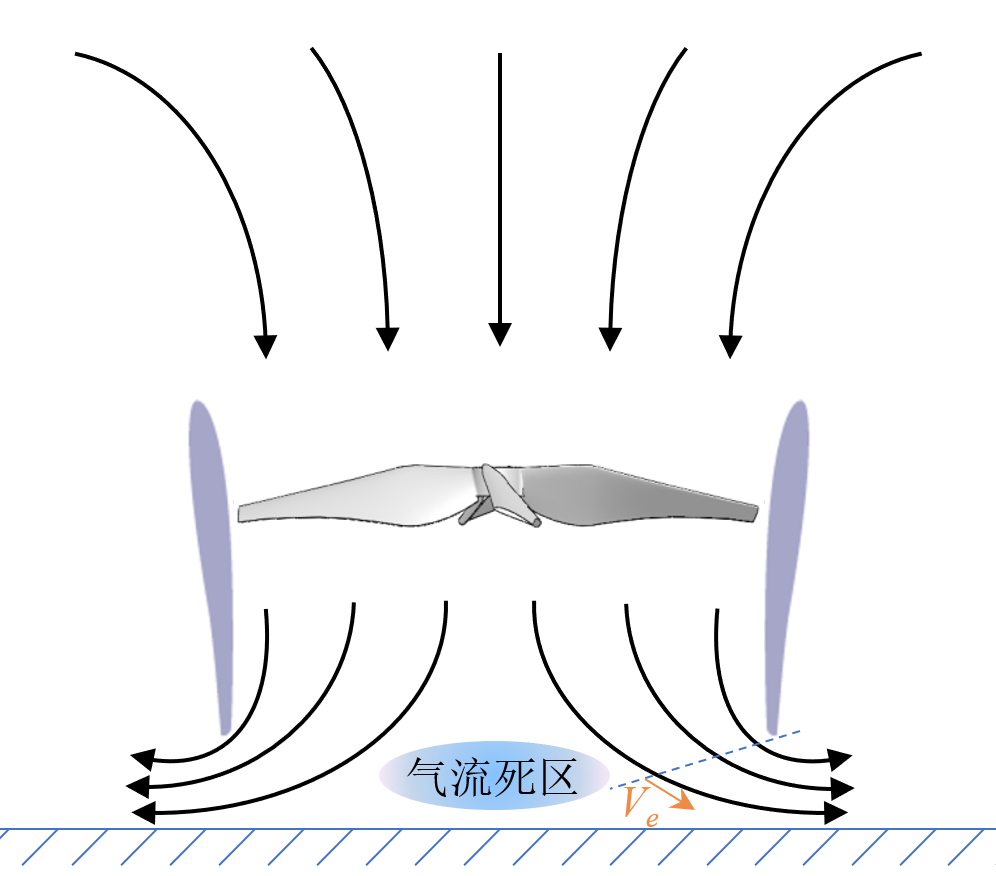
\includegraphics[scale=0.3]{figure/chapter4/ground_effect_flow.png}
\caption{地面效应下气体流动示意图}
\label{fig:flow_ground_effect}
\end{figure}

如图\ref{fig:flow_ground_effect}所示，当无人机在近地面工作时，从涵道出口排出的高速气流撞击地面后，会向四周扩散并形成径向射流。在此过程中，靠近涵道出口中心的下洗气流因地面阻塞而形成流速极低的“死水区”，导致有效气流面积减小，气流结构紊乱，进而致使控制舵面产生的有效偏转力下降。这种流场结构的改变是地面效应影响控制力矩的主要物理机制。

尽管近地面流场相对紊乱，但可以合理假设：在相同的气流环境下，单个舵面能够产生的升力仍与其偏转角度大致成线性关系。这是因为对于小角度偏转的控制舵面而言，其升力系数在一定的攻角范围内近似为线性，而地面效应主要通过改变当地气流速度和动压来影响升力大小，并不改变其与偏转角之间的线性本质。基于此，引入控制力衰减系数 $C_{cvGE}$ 来描述地面效应对舵面升力的影响，该系数仅与无量纲高度 $h/R$ 相关。则地面效应下单个舵面产生的偏转力 $F_{cvGE_i}$ 可表示为：
\begin{equation}
F_{cvGE_i} = C_{cvGE} F_{cv_i},
\label{eq:F_cvGE}
\end{equation}
其中 $F_{cv_i}$ 为无地效状态下相同舵面偏转角对应的偏转力。由式\eqref{eq:F_cv}以及表\ref{tab:lumped_parameters}可知，无地效状态下单个舵面的偏转力可表示为：
\begin{equation}
F_{cv_i} = K_{cv} \delta_i,
\end{equation}
式中 $K_{cv}$ 为无地效时的控制舵面偏转力系数，$\delta_i$ 为舵面偏转角。将上式代入式\eqref{eq:F_cvGE}可得：
\begin{equation}
F_{cvGE_i} = C_{cvGE} K_{cv} \delta_i = K_{cvGE} \delta_i,
\label{eq:F_cvGE_linear}
\end{equation}
其中 $K_{cvGE}$ 为地面效应下的控制舵面偏转力系数，满足：
\begin{equation}
K_{cvGE} = C_{cvGE} K_{cv}.
\label{eq:KcvGE}
\end{equation}
根据式\eqref{eq:M_cv}及表\ref{tab:lumped_parameters}中关于舵面偏转力系数的表达式，可得：
\begin{equation}
    M_{z}^b = K_{cvGE} l_2 (\delta_1 + \delta_2 + \delta_3 + \delta_4),
    \label{eq:M_cv_GE}
\end{equation}
其中 $l_2$ 为控制舵面压心到机体坐标系 $O_bZ_b$ 轴的距离。该式表明，在忽略舵面间气动干扰的理想情况下，总控制力矩与各舵面偏转角之和呈线性关系，比例系数即为地面效应下的偏转力系数 $K_{cvGE}$。

为准确获取 $K_{cvGE}$ 随高度的变化规律，本文设计了专门的静态台架实验。实验中将无人机倒置安装于六轴力/力矩传感器上，使涵道风扇轴线垂直于地面。在此安装方式下，传感器可直接测量由舵面偏转产生的绕机体坐标系 $O_bZ_b$ 轴的纯力矩分量，而涵道风扇产生的推力和侧向力对该力矩测量通道的影响可忽略不计。因此，通过该实验设置能够将控制力矩与其他气动力矩解耦，从而直接、准确地测量 $K_{cvGE}$。

由式\eqref{eq:KcvGE}可知，$K_{cvGE}$ 随高度的变化完全由衰减系数 $C_{cvGE}$ 决定。考虑到地面效应的物理特性：当无人机远离地面时，地面效应的影响应趋近于零，即 $C_{cvGE} \to 1$；随着离地高度减小，地面效应对舵面气流的阻塞和扰动作用增强，舵面偏转力随之衰减，即 $C_{cvGE}$ 逐渐减小。基于上述物理约束，并借鉴推力模型中广泛采用的指数衰减形式，假设衰减系数 $C_{cvGE}$ 满足如下关系：
\begin{equation}
C_{cvGE} = 1 - C_{cvAmp} \cdot e^{C_{cvExp} \cdot (h/R)},
\label{eq:CcvGE_model}
\end{equation}
其中 $C_{cvAmp}$ 为幅值系数，控制地面效应的最大衰减程度；$C_{cvExp}$ 为指数衰减系数，控制衰减随高度增加的速率。该模型形式简洁，且满足边界条件：当 $h/R \to \infty$ 时，$C_{cvGE} \to 1$；当 $h/R$ 减小时，$C_{cvGE}$ 呈指数下降，物理意义明确。该假设的合理性将通过后续实验结果进行验证，并基于实验数据辨识模型参数 $C_{cvAmp}$ 和 $C_{cvExp}$。

\section{实验平台} % 1 Page
\label{sec:exp_platform}
为准确获取涵道式无人机在地面效应影响下的执行器效率与控制力矩特性，并为第\ref{sec:model_identification}节中的参数拟合提供可靠的实验数据，本文搭建了一套基于多轴力/力矩传感器的变高度静态测试台架。通过该平台开展的静态台架实验，旨在完成对涵道风扇推力效益及控制舵面力矩效益的地面标定，从而建立地面效应下执行器控制效益的数学模型。

\begin{figure}
    \centering
    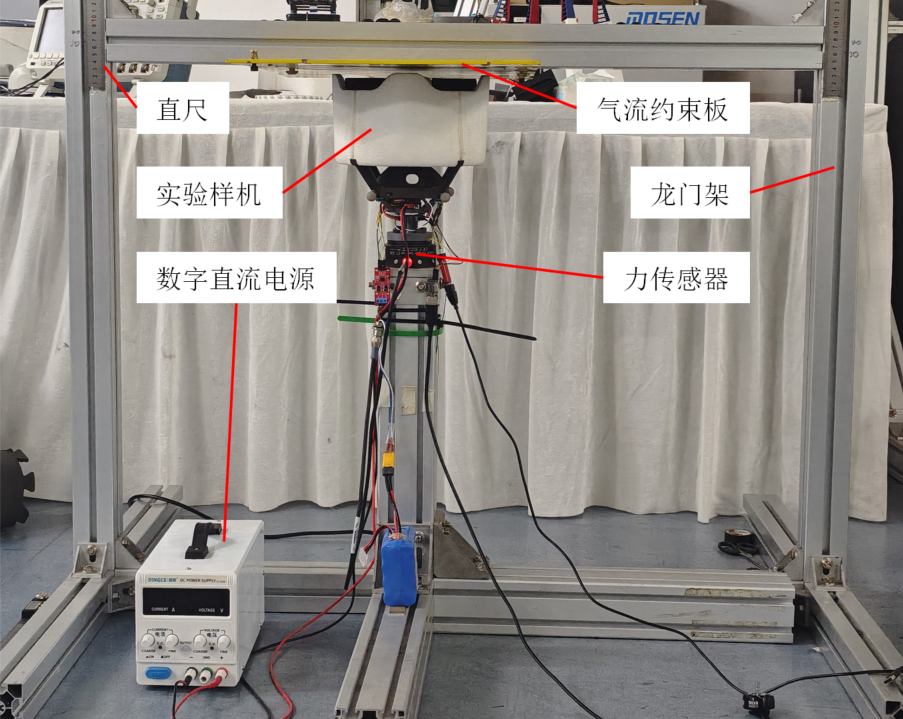
\includegraphics[width = 0.65\textwidth]{figure/chapter4/ground_effect_platform.png}
    \caption{\label{fig:experiment_platform}地面效应数据采集实验平台}
\end{figure}

实验平台的机械结构如图\ref{fig:experiment_platform}所示。台架主体采用铝合金型材搭建，具有足够的结构刚度以保证测试过程中的稳定性。上方采用龙门架结构固定一块面积远大于涵道风扇出口截面的刚性约束板，用于模拟真实的地面。该约束板可沿固定在龙门架两侧的精密竖直导轨平稳滑动，以精确调节其与涵道风扇之间的垂直距离。导轨上附有高精度直尺，用于记录每次数据采集时的约束板位置，从而确定离地高度。为保证实验数据的准确性与可重复性，实验中对离地高度$h$作如下定义：无人机底部支撑脚所在平面至约束板上表面的垂直距离。实验涵盖的无量纲高度范围为$0.2 \leq h/R \leq 4.0$，其中$R$为涵道风扇半径，该范围完整覆盖了从强地面效应区到无地效区的过渡。

实验样机以倒置姿态固定于测试台架上。具体而言，无人机机身通过专用夹具与下方的六维力/力矩传感器刚性连接，传感器则固定于底部基座上。采用倒置安装方式可使涵道风扇产生的推力垂直向上作用于传感器，便于直接测量。为准确获取螺旋桨的真实转速，排除了因供电电压波动或电机个体差异导致的转速不确定性，实验中使用高精度无刷电机转速传感器实时采集电机的电频率信号，并换算为螺旋桨的机械转速。整个实验系统由可编程数字直流电源供电，确保在长时间、多工况的测试过程中，供电电压保持稳定，从而保证电机工况的一致性和传感器数据的可靠性。

力/力矩传感器是本次实验的核心测量设备。根据实验样机在悬停及近地面工况下的预估最大推力与力矩，选用了量程合适、精度满足要求的传感器型号。传感器可同时测量三轴力与三轴力矩，其采样频率设置为$200\,\mathrm{Hz}$。这一采样频率，使得后期数据处理时可通过时域平均有效滤除高频噪声与气流脉动带来的随机误差，从而获得高精度的稳态气动力数据。

通过上述实验平台，可开展两类核心测试：一是地面效应下的涵道风扇推力效益测试，旨在获取不同离地高度下风扇推力相对于无地效状态的增益或损失；二是地面效应下的控制舵面力矩效益测试，旨在获取不同离地高度下各舵面单位偏角所产生的控制力矩。两类实验的具体步骤与数据处理方法将在后续章节详述。

\section{地面效应下涵道风扇推力模型辨识}
\label{sec:GE_exp}
为准确获取涵道风扇在地面效应影响下的推力特性，并为第\ref{subsec:thrust_model}节所建模型的参数辨识提供可靠的数据支撑，本节详细阐述地面效应下涵道风扇推力效益测试的实验步骤。实验基于第\ref{sec:exp_platform}节所述的多轴力/力矩传感器测试平台开展，通过系统性地改变离地高度与螺旋桨转速，采集相应的推力数据。

\subsection{实验步骤}

\textbf{1. 实验准备与传感器校准}

实验准备阶段，首先对测试平台进行校准与初始化。将涵道式无人机样机通过专用夹具倒置固定于六维力/力矩传感器之上，确保无人机机体轴线与传感器测量轴线对齐，且涵道出口平面保持水平。由于力传感器存在固有的静态零点误差，且无人机自身的重量会通过传感器输出一个恒定的偏置，该偏置将叠加在螺旋桨与控制舵面产生的气动力上，从而影响测量结果的准确性。为消除上述影响，在每次正式实验开始前，均需采集一组静态数据：在无人机未通电、螺旋桨静止的状态下，以采样频率 $200\mathrm{Hz}$ 连续记录力/力矩传感器输出 $5\mathrm{s}$，并将该段时间内各通道测量值的平均值作为该次实验的静态零点与自重偏置值。该偏置值将在后续数据处理中予以扣除，以消除传感器零点漂移和无人机自重对测量结果的影响。静态校准数据记录于飞控板载SD卡中。

\textbf{2. 实验工况设定}

实验的独立变量包括无量纲高度 $h/R$ 和螺旋桨转速 $\Omega$。无量纲高度 $h/R$ 的设定范围需完整覆盖地面效应的主要影响区间。根据第\ref{subsec:thrust_model}节的分析，涵道风扇的地面效应在 $h/R < 4.0$ 时显著，而当 $h/R > 4.0$ 时可视为无地效区。同时，为避免进入 $h/R < 0.2$ 的极端近地失速区，实验高度范围设定为 $h = 10\mathrm{mm}$ 至 $400\mathrm{mm}$，对应无量纲高度 $h/R$ 分别为：$0.1124$、$0.2247$、$0.3371$、$0.4494$、$0.5618$、$0.6742$、$0.7865$、$0.8989$、$1.0112$、$1.1236$、$1.2360$、$1.6854$、$2.2472$、$3.3708$、$4.4944$。其中，$h = 10\mathrm{mm}$ 对应强地面效应区，$h = 400\mathrm{mm}$ 对应无地效边界。实验过程中，通过调节龙门架上的竖直导轨，将约束板依次固定至上述各高度位置，并使用附带的直尺精确读取并记录当前离地高度。

螺旋桨转速范围的确定以无人机典型悬停状态为基准。根据前期飞行测试，本文所用样机在 $h/R > 4.0$ 的无地效环境中，稳定悬停所需的螺旋桨转速约为 $\Omega_{\mathrm{hover}} = 790\mathrm{rad/s}$。为充分覆盖悬停及低速机动工况下的推力特性，并保证数据对模型参数辨识的有效性，将转速范围设定为悬停转速的 $\pm 10\%$，即 $\Omega \in [710,870]\mathrm{rad/s}$。在该范围内均匀选取 $12$ 个转速点作为测试工况。对于每个固定的离地高度 $h$，均遍历上述所有转速点，以获取推力随转速变化的完整曲线。

\textbf{3. 数据采集流程}

具体实验操作流程如下：首先将约束板调整至目标高度并锁紧。随后，通过数字直流电源向电机电调系统供电，并按照预设的油门指令序列由低到高依次驱动螺旋桨达到各目标转速。在每个油门指令发出后，等待 $2\mathrm{s}$，以使得电机转速建立稳态，并消除启动瞬态过程对测量的影响。待螺旋桨旋转稳定后，以 $200\mathrm{Hz}$ 的采样频率连续记录力/力矩传感器的输出数据，记录时长不少于 $5\mathrm{s}$，以保证后续统计平均处理时能够有效滤除高频气动噪声与机械振动干扰。记录过程中，同步采集无刷电机测速模块输出的转速信号，以确认实际转速与指令转速的一致性。完成该高度下所有转速点的测量后，将约束板调整至下一高度，重复上述过程。

所有实验数据均通过飞控板载的微控制器实时采集，并存储于机载SD卡中。数据记录的内容包括：时间戳、六维力/力矩传感器各通道原始数值、螺旋桨转速反馈值、当前离地高度以及对应的油门指令。实验结束后，将SD卡中的数据导出至计算机，供后续的数据预处理与参数拟合使用。为保证实验结果的可靠性与可重复性，每个工况（特定高度与转速的组合）均重复测量三次，取三次测量的平均值作为该工况下的最终推力值，以降低随机误差的影响。

\textbf{4. 数据预处理}

实验完成后，从SD卡中导出原始数据，按以下步骤进行预处理：

首先，对每一组测量工况（固定的 $h/R$ 与 $\Omega$），取 $5\mathrm{s}$ 采样窗口内的力/力矩数据进行算术平均，得到该工况下的稳态推力测量值。这一处理可有效抑制传感器高频噪声及气流脉动对测量结果的影响。

其次，将每一组稳态推力测量值减去实验前采集的静态零点偏置值，得到净气动力 $T_{GE}$。该值即反映了涵道风扇产生的净推力。

最后，将处理后的数据按 $h/R$ 和 $\Omega$ 进行整理，形成用于后续参数辨识的样本数据集。

\subsection{实验数据} % 2 Pages
\label{subsec:thrust_exp}
按照第\ref{subsec:thrust_exp}节所述的实验步骤完成数据采集与预处理后，可得到涵道风扇推力 $T$ 与无量纲高度 $h/R$ 以及螺旋桨转速 $\Omega$ 之间的映射关系。图\ref{fig:T-omega-h}以三维曲面的形式展示了该关系的全貌，其中横轴分别为无量纲高度 $h/R$ 与螺旋桨转速的平方 $\Omega^2$，纵轴为推力 $T{GE}$，曲面上叠加的白色曲线为等高线，颜色由黄色渐变至蓝色用以表示推力大小，黄色区域对应推力较大，蓝色区域对应推力较小。

\begin{figure}
    \centering
    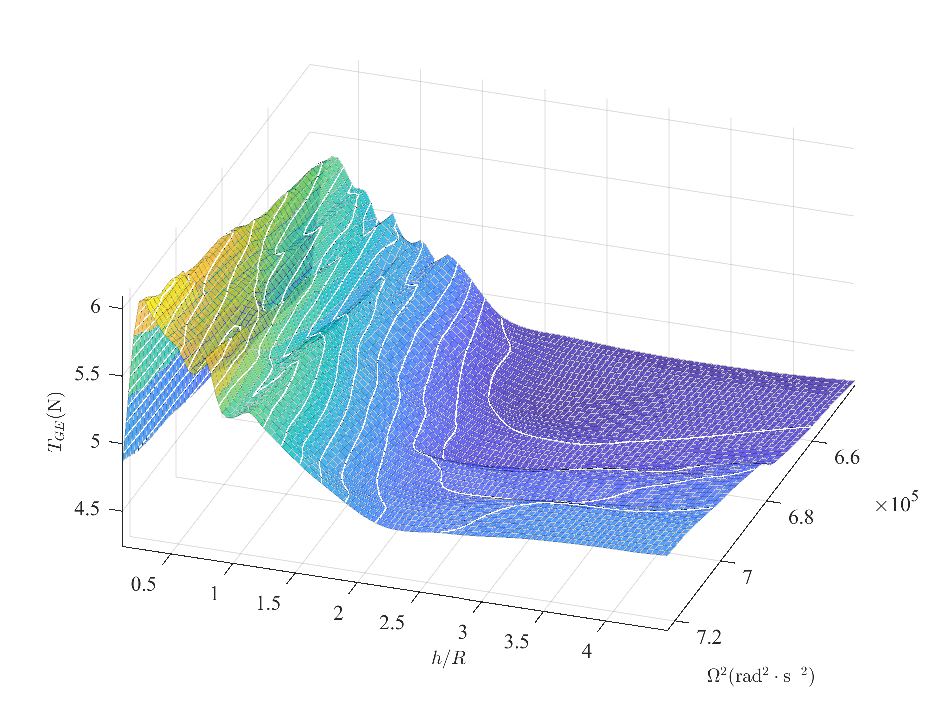
\includegraphics{matlab/ground_effect/pdf/thrust/surf_T-omega-h.pdf}
    \caption{\label{fig:T-omega-h}涵道风扇推力和风扇转速、离地高度之间的关系}
\end{figure}

从整体趋势观察，推力随无量纲高度 $h/R$ 的变化呈现非单调特性：当无人机从高空下降时，推力首先逐渐增大，在 $h/R \approx 0.25$ 附近达到峰值，随后随高度进一步降低而迅速减小。这一变化规律与现有文献中关于涵道风扇地面效应的研究结论相符。文献\cite{luo2023numerical}通过CFD仿真发现，地面效应下涵道风扇总推力的变化是桨叶推力与涵道推力此消彼长的结果：当地面接近时，出口射流受阻形成高压区，桨叶推力显著增加，但同时涵道唇口处的低压区被削弱，涵道推力大幅下降。当高度比降至 $h/R < 0.5$ 时，涵道推力下降占主导地位，导致总推力出现损失。此外，当 $h/R < 0.2$ 时，叶片尖端发展出大量失速涡胞，流场呈现强烈的非定常特性，推力急剧下降且波动剧烈\cite{luo2023numerical}，该区域不在本文推力模型的有效拟合范围内。在 $h/R > 2.0$ 的范围内，地面效应逐渐减弱，推力缓慢趋近于无地效状态下的基准值，这与文献\cite{Antonio2021}中关于旋翼地效影响范围 $h/R \leq 2.0$ 的结论基本吻合。

为深入分析推力特性与各变量之间的依赖关系，本文从两个维度对实验数据进行剖面分析。

\begin{figure}[htbp]
    \centering
    \begin{minipage}[b]{0.45\textwidth}
        \centering
        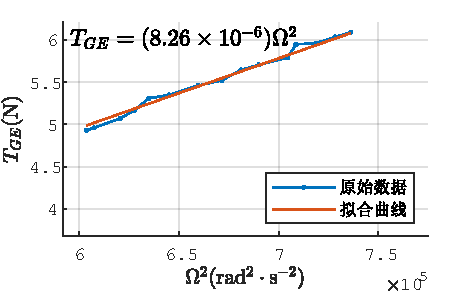
\includegraphics{matlab/ground_effect/pdf/thrust/rotor_thrust_30mm.pdf}
        \caption*{a. $h/R = 0.34$}
    \end{minipage}
    \hfill  % 产生弹性水平间距
    \begin{minipage}[b]{0.45\textwidth}
        \centering
        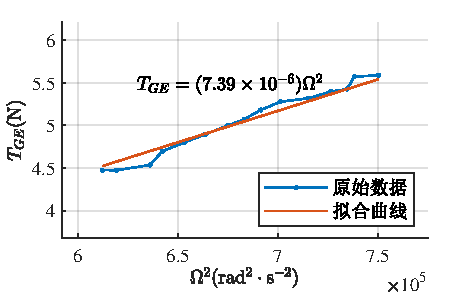
\includegraphics{matlab/ground_effect/pdf/thrust/rotor_thrust_100mm.pdf}
        \caption*{b. $h/R = 1.12$}
    \end{minipage}

    \vspace{0.5cm}

    \centering
    \begin{minipage}[b]{0.45\textwidth}
        \centering
        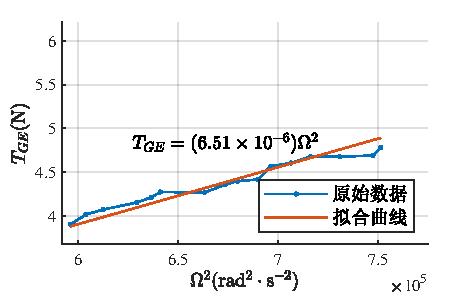
\includegraphics{matlab/ground_effect/pdf/thrust/rotor_thrust_200mm.pdf}
        \caption*{c. $h/R = 2.25$}
    \end{minipage}
    \hfill  % 产生弹性水平间距
    \begin{minipage}[b]{0.45\textwidth}
        \centering
        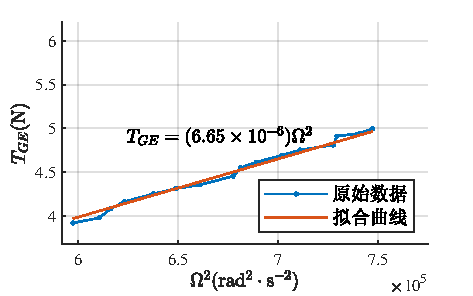
\includegraphics{matlab/ground_effect/pdf/thrust/rotor_thrust_400mm.pdf}
        \caption*{d. $h/R = 4.49$}
    \end{minipage}
    \caption{\label{fig:T-Omega}不同高度比$h/R$下推力$T$与风扇转速的平方$\Omega^2$的关系}
\end{figure}

首先，固定无量纲高度 $h/R$，考察推力 $T_{GE}$ 与螺旋桨转速平方 $\Omega^2$ 之间的关系。图\ref{fig:T-Omega}选取了四个典型高度比 $h/R = 0.34$、$1.12$、$2.25$ 和 $4.49$ 下的实验结果。图中浅蓝色带点标记的实线为该高度下的实测推力均值，橙色实线为通过最小二乘法拟合的正比例关系线，拟合式标注于曲线旁。可见，在不同高度比下，推力 $T_{GE}$ 与 $\Omega^2$ 之间均呈现良好的线性关系。这一结果验证了第\ref{subsec:thrust_model}节所建立推力模型的合理性，即地面效应下的推力可表示为无地效推力与一个仅与高度相关的衰减系数的乘积，如式\eqref{eq:GE_thrust_model}所示。此外，对比不同高度下的拟合直线可以发现：随着 $h/R$ 增大，推力 $T_{GE}$ 整体下降，且 $T$ 对 $\Omega^2$ 的斜率（即推力系数）也随之减小，这反映了地面效应衰减程度随高度增加而减弱的物理规律。

\begin{figure}
    \centering
    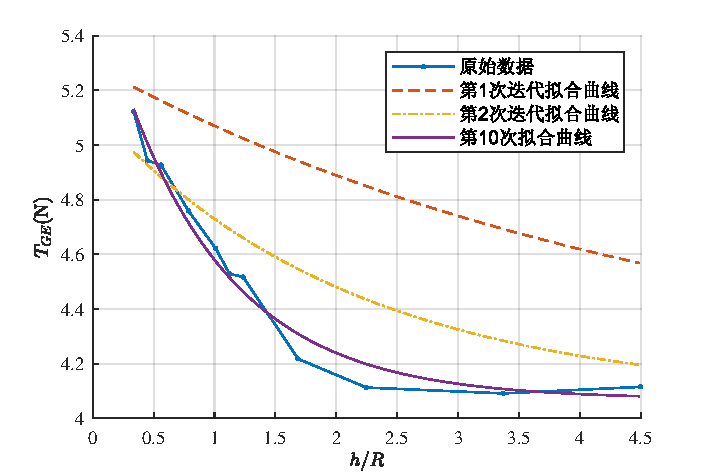
\includegraphics{matlab/ground_effect/pdf/thrust/line_T-h.pdf}
    \caption{\label{fig:T-h}典型工作转速下涵道风扇推力$T$和离地高度比$h/R$的关系}
\end{figure}

其次，固定螺旋桨转速为典型工作转速 $\Omega = 790\,\mathrm{rad/s}$（即无地效悬停转速），考察推力 $T_{GE}$ 与无量纲高度 $h/R$ 之间的关系。图\ref{fig:T-h}展示了该工况下的实验数据，其中浅蓝色带点标记的实线为实测推力均值。从图中可以看出，推力随高度增加呈现快速衰减后缓慢趋近于稳定值的趋势：当 $h/R < 1.0$ 时，推力随高度上升迅速下降；当 $h/R$ 介于 $1.0$ 至 $2.0$ 之间时，推力下降速度减缓；当 $h/R > 2.0$ 时，推力变化趋于平缓，并逐渐趋近于无地效状态下的基准推力 $T_{df} \approx 4.07\,\mathrm{N}$。这一变化趋势与第\ref{subsec:thrust_model}节提出的指数衰减模型高度吻合，为后续模型参数的辨识提供了可靠的数据基础。

综合上述两个维度的分析，可以得出以下结论：地面效应对涵道风扇推力的影响主要体现在对推力系数的调制上，推力与转速平方的线性关系在不同高度下均成立；推力随高度变化的衰减规律呈现指数特性，在 $h/R < 0.5$ 时存在推力损失峰值区，在 $h/R > 2.0$ 时地面效应基本可忽略。这些实验数据将为第\ref{subsec:thrust_fitting}节的模型参数辨识提供直接的依据。

\subsection{参数拟合}
\label{subsec:thrust_fitting}

利用第\ref{subsec:thrust_exp}节所获取的典型工作转速（$\Omega = 790\,\mathrm{rad/s}$）下各无量纲高度 $h/R$ 对应的平均推力数据，对第\ref{subsec:thrust_model}节建立的推力模型进行参数辨识。由于模型为非线性形式，无法直接应用线性最小二乘法，本文采用高斯-牛顿迭代法求解待定参数。

由式\eqref{eq:ge_coefficient}和式\eqref{eq:GE_thrust_model}可知，地面效应下的推力 $T_{GE}$ 与参数 $C_{TAmp}$、$C_{TExp}$ 之间的关系为：
\begin{equation}
    T_{GE} = T_{df}\left(1 + C_{TAmp} \cdot e^{C_{TExp} \cdot (h/R)}\right),
    \label{eq:thrust_fit_model}
\end{equation}
其中 $T_{df}$ 为无地效状态下的推力基准值，通过无遮挡环境下测量得到，本文实测值为 $T_{df} = 4.07\,\mathrm{N}$。

记第 $i$ 次采集的平均推力值为 $T_{GE,i}$，对应无量纲高度为 $h_i/R$，$i = 1,2,\dots,n$，$n$ 为数据点数。定义拟合误差为：
\begin{equation}
    E_{TGE,i} = T_{GE,i} - T_{df}\left(1 + C_{TAmp} \cdot e^{C_{TExp} \cdot (h_i/R)}\right),\quad i = 1,2,\dots,n.
\end{equation}

参数拟合的目标是求取使误差平方和最小的参数组合，即求解如下优化问题：
\begin{equation}
    \min_{C_{TAmp}, C_{TExp}} \quad \sum_{i=1}^{n} E_{TGE,i}^2.
    \label{eq:ls_obj}
\end{equation}

定义误差向量 $\boldsymbol{E}_{TGE} \in \mathbb{R}^{n}$ 为：
\begin{equation}
    \boldsymbol{E}_{TGE} = [E_{TGE,1}, E_{TGE,2}, \dots, E_{TGE,n}]^{T}.
\end{equation}
根据高斯-牛顿法，在第 $k$ 次迭代时，需计算误差向量关于参数的雅可比矩阵 $\boldsymbol{J}_T^{(k)} \in \mathbb{R}^{n \times 2}$，其元素为：
\begin{equation}
    \boldsymbol{J}_T^{(k)} = 
    \begin{bmatrix}
        \dfrac{\partial E_{TGE,1}}{\partial C_{TAmp}} & \dfrac{\partial E_{TGE,1}}{\partial C_{TExp}} \\[6pt]
        \vdots & \vdots \\[6pt]
        \dfrac{\partial E_{TGE,n}}{\partial C_{TAmp}} & \dfrac{\partial E_{TGE,n}}{\partial C_{TExp}}
    \end{bmatrix}_{\boldsymbol{\theta}=\boldsymbol{\theta}^{(k)}},
\end{equation}
其中偏导数的具体表达式为：
\begin{equation}
    \begin{cases}
        \dfrac{\partial E_{TGE,i}}{\partial C_{TAmp}} = -T_{df} \, e^{C_{TExp} \cdot (h_i/R)},\\[8pt]
        \dfrac{\partial E_{TGE,i}}{\partial C_{TExp}} = - (h_i/R)\, T_{df}\, C_{TAmp} \, e^{C_{TExp} \cdot (h_i/R)}.
    \end{cases}
    ,\quad i = 1,2,\dots,n.
\end{equation}

高斯-牛顿迭代法中的迭代步长 $\boldsymbol{\delta}_T^{(k)} = [\Delta C_{TAmp}, \Delta C_{TExp}]^{T}$ 由正规方程确定：
\begin{equation}
    \boldsymbol{\delta}_T^{(k)} = -\left( (\boldsymbol{J}_T^{(k)})^{T} \boldsymbol{J}_T^{(k)} \right)^{-1} (\boldsymbol{J}_T^{(k)})^{T} \boldsymbol{E}_{TGE}^{(k)}.
\end{equation}
参数更新公式为：
\begin{equation}
    \boldsymbol{\theta}_T^{(k+1)} = \boldsymbol{\theta}_T^{(k)} + \boldsymbol{\delta}_T^{(k)},
\end{equation}
其中 $\boldsymbol{\theta}_T^{(k)} = [C_{TAmp}^{(k)}, C_{TExp}^{(k)}]^{T}$。该迭代算法在收敛点附近具有二次收敛速度。

本文选取参数初始值 $C_{TAmp}^{(0)} = 0.3$，$C_{TExp}^{(0)} = -0.25$，共执行 $10$ 次迭代。第$1$次，第$2$次以及第$10$次迭代的拟合结果如图\ref{fig:T-h}所示。迭代过程中参数的收敛曲线如图\ref{fig:T_param-iter}所示，误差平方和 $\sum E_{TGE,i}^2$ 随迭代次数的变化如图\ref{fig:T_err_iter}所示。

\begin{figure}[htbp]
    \centering
    \begin{minipage}[b]{0.45\textwidth}
        \centering
        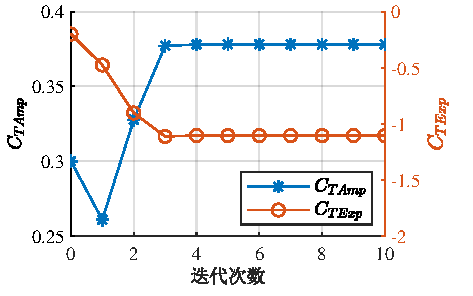
\includegraphics{matlab/ground_effect/pdf/thrust/T_param-iter.pdf}
        \caption{拟合参数与迭代次数的关系}
        \label{fig:T_param-iter}
    \end{minipage}
    \hfill
    \begin{minipage}[b]{0.45\textwidth}
        \centering
        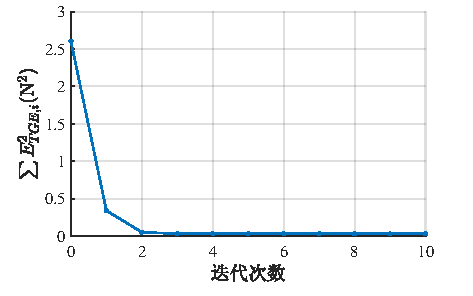
\includegraphics{matlab/ground_effect/pdf/thrust/T_err_iter.pdf}
        \caption{拟合误差平方和与迭代次数的关系}
        \label{fig:T_err_iter}
    \end{minipage}
\end{figure}

从图中可以看出，经过 $3$ 次迭代后，拟合参数已基本趋于稳定，误差平方和迅速减小至初始值的 $1.1\%$，表明算法收敛速度较快。最终收敛得到的参数值为：
\begin{equation}
    C_{TAmp} = 0.378,\qquad C_{TExp} = -1.105.
\end{equation}
将上述参数代入式\eqref{eq:thrust_fit_model}，并结合无地效推力基准值 $T_{df} = 4.07\,\mathrm{N}$，可得地面效应下涵道风扇推力模型的具体表达式为：
\begin{equation}
    T_{GE} = 4.07\left(1 + 0.378 \cdot e^{-1.105 \cdot (h/R)}\right),
    \label{eq:fitted_thrust_model}
\end{equation}
其中 $T_{GE}$ 单位为$\mathrm{N}$。该模型的拟合曲线已在图\ref{fig:T-h}中以紫色实线形式给出，与实验数据吻合良好，验证了所提指数模型能够准确描述涵道风扇推力随离地高度的变化规律。该模型将在后续章节中用于近地面抗扰控制器的设计与补偿。

\section{地面效应下控制舵面偏转力模型辨识}
\label{sec:cv_identification}

为准确获取涵道式无人机在地面效应影响下的控制舵面偏转力特性，并为第\ref{subsec:cv_model}节所建控制力矩模型中的衰减系数 $C_{cvGE}$ 提供参数辨识依据，本节开展地面效应下的控制舵面力矩效益测试。根据第\ref{subsec:cv_model}节的理论推导，地面效应下的控制力矩与舵面偏转角之和呈线性关系，比例系数 $K_{cvGE}$ 反映了舵面偏转力的综合效益。本实验旨在通过静态台架测量，获取不同离地高度下 $K_{cvGE}$ 随高度变化的规律，进而辨识衰减系数 $C_{cvGE}$ 中的待定参数。

实验的核心思路是利用无人机的结构对称性与倒置安装方式实现力矩测量的解耦。如第\ref{subsec:cv_model}节所述，当四个控制舵面输出相同的偏转角度 $\delta_c$ 时，由于结构对称性，处于对侧的舵面所产生的偏转力大小相等、方向相反，其绕机体坐标系 $O_bX_b$ 轴和 $O_bY_b$ 轴的力矩分量相互抵消。在此条件下，六维力/力矩传感器测量得到的绕 $O_bZ_b$ 轴的扭矩，可近似认为完全由四个舵面偏转力对该轴的力矩贡献构成，从而排除了其他气动力矩的干扰。基于此，通过测量不同高度下气动力扭矩 $M_{z}^b$ 与舵面偏转角 $\delta_c$ 的关系，即可直接辨识出地面效应下的偏转力系数 $K_{cvGE}$。

实验基于第\ref{sec:exp_platform}节所述的多轴力/力矩传感器测试平台开展。实验样机以倒置姿态固定，涵道风扇轴线垂直于地面。通过系统性地改变离地高度与舵面偏转角度，采集相应的扭矩数据，为后续模型参数辨识提供可靠的数据支撑。

\subsection{实验步骤}
\label{subsec:torque_exp}

\textbf{1. 实验准备与传感器校准}

与推力测试实验相同，在正式实验开始前，需完成力/力矩传感器的静态校准。将涵道式无人机样机通过专用夹具倒置固定于六维力/力矩传感器之上，确保无人机机体轴线与传感器测量轴线对齐，且涵道出口平面保持水平。在无人机未通电、螺旋桨静止、舵面无偏转的状态下，以 $200\,\mathrm{Hz}$ 的采样频率连续采集力/力矩传感器输出 $5\,\mathrm{s}$，并将该段时间内各通道测量值的平均值作为该次实验的静态零点与自重偏置值。该偏置值将在后续数据处理中予以扣除，以消除传感器零点漂移和无人机自重对测量结果的影响。静态校准数据记录于飞控板载SD卡中。

\textbf{2. 实验工况设定}

实验的独立变量包括无量纲高度 $h/R$ 和舵面偏转角 $\delta_c$。无量纲高度 $h/R$ 的设定范围与推力测试实验保持一致，涵盖从强地面效应区到无地效区的完整过渡。通过调节龙门架上的竖直导轨，将约束板依次固定至各高度位置，并使用附带的直尺精确读取并记录当前离地高度。

螺旋桨转速设定为典型悬停转速 $\Omega = 790\,\mathrm{rad/s}$，该转速与推力测试实验中的典型工作转速一致，以确保舵面所处的气流环境与实际飞行工况相符。通过数字直流电源向电机电调系统供电，并维持该转速稳定。

舵面偏转角度 $\delta_c$ 的设定需覆盖控制舵面的有效线性工作范围。根据第\ref{subsec:cv_dynamics}节的分析，舵面偏转角应限制在 $\delta_i \in [-20^\circ, 20^\circ]$ 范围内以保证气动力的线性特性。在实验中，令四个舵面同时输出相同的偏转角度 $\delta_c$，并在$[-20^\circ, 20^\circ]$范围内以$2^\circ$为步长，均匀选取 $21$ 个角度点。对于每个固定的离地高度 $h$，均遍历上述所有舵面偏转角度。

\textbf{3. 数据采集流程}

具体实验操作流程如下：首先将约束板调整至目标高度并锁紧，通过数字直流电源向电机电调系统供电，使螺旋桨达到并稳定在典型悬停转速 $\Omega = 790\,\mathrm{rad/s}$。待电机转速稳定 $2\,\mathrm{s}$ 后，飞控系统按照预设的舵面偏转角度序列，依次驱动四个舵面同步偏转至目标角度 $\delta_c$。每个舵面偏转角度维持输出 $10\,\mathrm{s}$，以保证气动状态达到稳态，并采集足够长度的数据用于后续统计平均处理。

在舵面维持统一偏转角度$\delta_c$的 $10\,\mathrm{s}$ 时间内，以 $200\,\mathrm{Hz}$ 的采样频率连续记录六维力/力矩传感器的输出数据，重点记录绕 $O_bZ_b$ 轴的扭矩分量 $M_{z}^b$。数据采集过程中，同步记录当前的无量纲高度 $h/R$ 与舵面偏转角 $\delta_c$。完成当前高度下所有舵面角度的测量后，将约束板调整至下一高度，重复上述过程。

所有实验数据均通过飞控板载的微控制器实时采集，并存储于机载SD卡中。数据记录的内容包括：时间戳、六维力/力矩传感器各通道原始数值、螺旋桨转速反馈值、当前离地高度以及舵面偏转角度指令。实验结束后，将SD卡中的数据导出至计算机，供后续的数据预处理与参数拟合使用。

\textbf{4. 数据预处理}

实验完成后，从SD卡中导出原始数据，按以下步骤进行预处理：

首先，对每一组测量工况（固定的 $h/R$ 与 $\delta_c$），取 $10\,\mathrm{s}$ 采样窗口内的绕 $O_bZ_b$ 轴扭矩数据进行算术平均，得到该工况下的稳态扭矩测量值。这一处理可有效抑制传感器高频噪声及气流脉动对测量结果的影响。

其次，将每一组稳态扭矩测量值减去实验前采集的静态零点偏置值，得到净气动力矩 $M_{z}^b$。该值即反映了舵面偏转产生的净控制力矩。

最后，将处理后的数据按 $h/R$ 和 $\delta_c$ 进行整理，形成用于后续参数辨识的样本数据集。

% \subsection{实验数据} % 2 Pages
% 将数据集整理成气动力矩$M_{z}^b$和高度$h/R$以及舵面偏转角度$\delta$之间的关系如图\ref{fig:moment-h-delta}所示。横轴为高度比和舵面偏转角度的平方，纵轴为沿机体轴的气动力矩$M_{z}^b$。并且使用渐变的黄色到蓝色以描述力矩大小，黄色力矩大，蓝色力矩小。

% \begin{figure}[htbp]
%     \centering
%     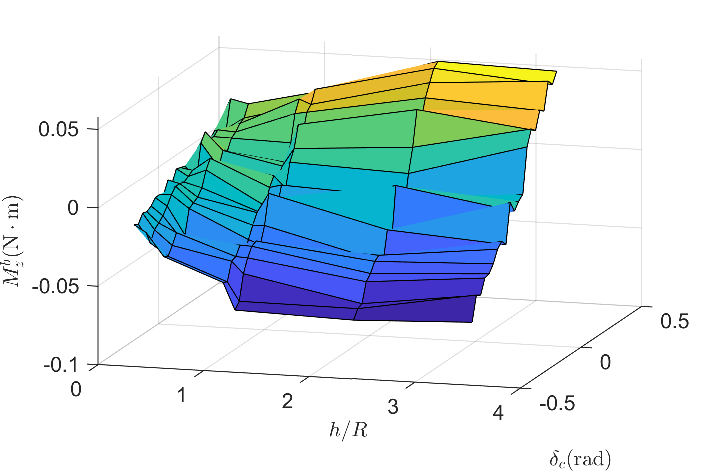
\includegraphics{figure/chapter4/moment-h-delta.pdf}
%     \label{fig:moment-h-delta}
% \end{figure}

% 整体趋势上来看，在同一高度下，气动力矩$M_{z}^b$与舵面偏转角呈现出正相关的关系。气动力矩$M_{z}^b$对舵面偏转角的斜率反映了控制舵面偏转力系数的大小，该斜率越大，表明气动力矩$M_{z}^b$受到舵面偏转角的影响越大。在$h/R < 2.0$时，随着无人机离地面高度的上升，该斜率不断上升，在$h/R > 2.0$后，逐渐远离地效区，该斜率趋于平缓。

% 本文从两个维度来深入分析该实验结果，分别是在指定高度下，气动力矩$M_{z}^b$随舵面角度$\delta$变化的曲线；以及在舵面角度为零时输出，气动力矩$M_{z}^b$随高度比的变化曲线。

% \begin{figure}[htbp]
%     \centering
%     \begin{minipage}[b]{0.45\textwidth}
%         \centering
%         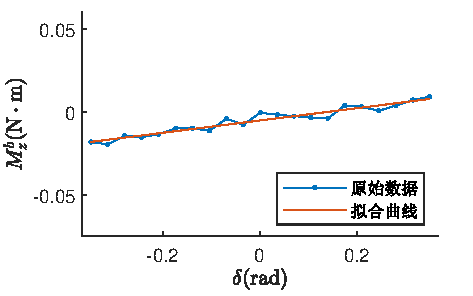
\includegraphics{figure/chapter4/cv_moment_15mm.pdf}
%         \caption*{$h/R = 0.17$}
%     \end{minipage}
%     \hfill  % 产生弹性水平间距
%     \begin{minipage}[b]{0.45\textwidth}
%         \centering
%         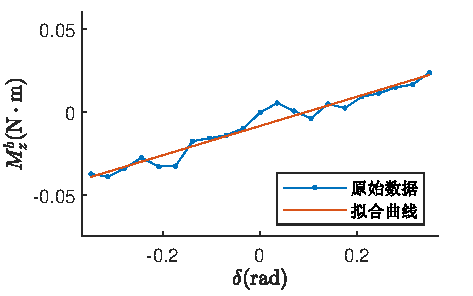
\includegraphics{figure/chapter4/cv_moment_40mm.pdf}
%         \caption*{$h/R = 0.45$}
%     \end{minipage}

%     \vspace{0.5cm}

%     \centering
%     \begin{minipage}[b]{0.45\textwidth}
%         \centering
%         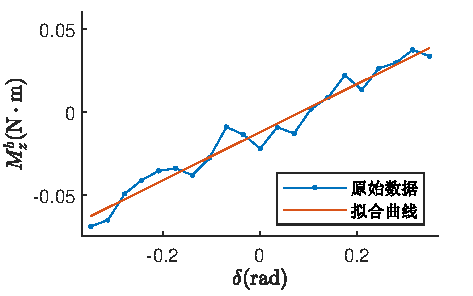
\includegraphics{figure/chapter4/cv_moment_100mm.pdf}
%         \caption*{$h/R = 1.12$}
%     \end{minipage}
%     \hfill  % 产生弹性水平间距
%     \begin{minipage}[b]{0.45\textwidth}
%         \centering
%         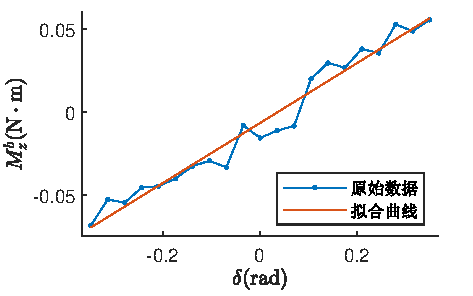
\includegraphics{figure/chapter4/cv_moment_300mm.pdf}
%         \caption*{$h/R = 3.36$}
%     \end{minipage}
%     \caption{不同高度比$h/R$下扭矩$M_z^b$与舵面角度$\delta$的关系}
%     \label{fig:cv_moment-delta}
% \end{figure}
% 在各高度下，分别对气动力矩$M_z^b$与舵面偏转角度$\delta$的关系作最小二乘拟合。设高度为$h_i$时，气动力矩$M_z^b$与舵面偏转角度$\delta$的最小二乘拟合线的斜率为$a_{i}$，截距为$b_{i}$。

% 在采集到的数据中，选取几个具有代表性的高度$(15mm, 40mm, 100mm, 30mm)$，分别对应高度比$(0.17, 0.45, 1.12, 3.36)$，将这几个高度下的气动扭矩$M_z^b$与舵面偏转角度的关系绘制于图\ref{fig:cv_moment-delta}中。其中浅蓝色带点标记的实线为实验数据，橙色线为线性关系最小二乘拟合线。

% 可见在不同高度比下，即使气流比较紊乱。气动扭矩$M_z^b$仍然与舵面偏转角度呈现出线性关系，这点与模型提出的假设所吻合。且随着离地高度$h_i$增加，$a_{i}$越来越大，反映出控制舵面偏转力系数$K_{cvGE}$与离地高度呈现出正相关关系，这也与模型\eqref{eq:CcvGE_model}相吻合。

% \begin{figure}[htbp]
%     \centering
%     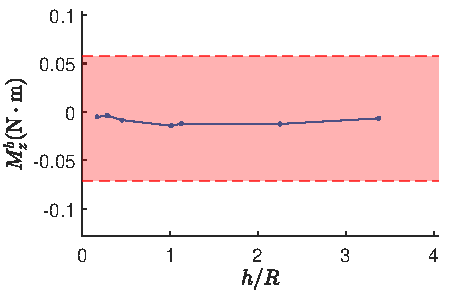
\includegraphics{figure/chapter4/zero_output_moment.pdf}
%     \caption{零输出时扭矩$M_z^b$与离地高度$h$的关系}
%     \label{fig:zero_output-moment}
% \end{figure}


% 将高度为$h_i$时的截距为$b_{i}$作为零输出时的受到的气动力矩$M_{z0}^b$。并整理出$M_{z0}^b$与高度比的关系如图\ref{fig:zero_output-moment}。其中浅蓝色带点标记的实线为各高度比下的气动扭矩，粉红色区域为无地面效应时，气动力矩的输出范围。

% 可见，在各高度下，无舵面偏转时的气动力矩$M_{z0}^b$并非为零，这是由于涵道风扇和反扭距襟翼都会产生沿机体轴的扭矩，由于加工，组装的误差，这两扭矩并未完全相互抵消，这一现象处于预期范围之内。
% 此外，$M_{z0}^b$随高度比的变化幅度仅占$M_z^b$随控制舵面变化的幅度的$7\%$，可见，$M_{z0}^b$受离地高度比的影响较小，本文不将该影响考虑在建模范围之内，认为$M_{z0}^b$为固定值。

% \begin{figure}[htbp]
%     \centering
%     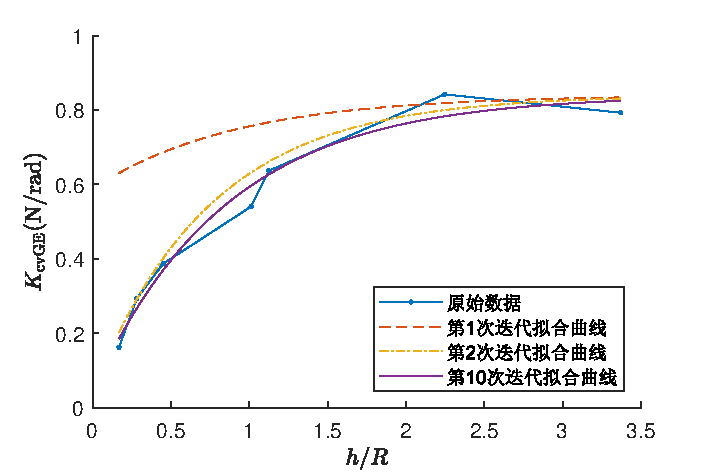
\includegraphics{figure/chapter4/K_cv-h.pdf}
%     \label{fig:K_cv-h}
% \end{figure}

% 根据控制舵面偏转力系数模型\eqref{eq:KcvGE_model}，拟合该模型需要各高度下$K_{cvGE}$和高度比$h/R$关系的数据。由式\eqref{eq:M_cv_GE}可知：
% \begin{equation}
%     K_{cvGE} = \frac{M_z^b}{l_2(\delta_1 + \delta_2 + \delta_3 + \delta_4)} = \frac{M_z^b}{4 l_2 \delta_c}
%     \label{eq:K_cvGE}
% \end{equation}
% 气动力矩$M_z^b$与舵面偏转角度$\delta$线性最小二乘斜率为$a_{i}$，那么由式\eqref{eq:K_cvGE}，高度为$h_i$时，可近似认为：
% \begin{equation}
%     K_{cvGE} = \frac{M_z^b}{4 l_2 \delta_c} \approx \frac{a_{i}}{4 l_2} = K_{cvGE,i}.
% \end{equation}
% 其中$K_{cvGE,i}$为通过$a_{i}$计算的，离地高度为$h_i$时的控制舵面偏转力系数。

% 各高度$h_i$与其对应的$K_{cvGE,i}$的关系如图\ref{fig:K_cv-h}所示。

% 在$h/R < 1.5$时，$K_{cvGE,i}$随着$h_i$的上升，迅速从$0.2$上升至$0.7$，随后，在$1.5 < h/R < 2.0$时，$K_{cvGE,i}$继续缓慢上升至$0.75$，在$h/R > 2.0$时，$K_{cvGE,i}$基本保持稳定。这与\ref{subsec:cv_model}小节提出的指数模型的趋势基本吻合。
\subsection{实验数据}

按照第\ref{subsec:torque_exp}节所述的实验步骤完成数据采集与预处理后，可得到控制舵面产生的气动力矩 $M_z^b$ 与无量纲高度 $h/R$ 以及舵面偏转角 $\delta$ 之间的映射关系。图\ref{fig:moment-h-delta}以三维曲面的形式展示了该关系的全貌，其中横轴分别为无量纲高度 $h/R$ 与舵面偏转角 $\delta$，纵轴为沿机体坐标系 $O_bZ_b$ 轴的气动力矩 $M_z^b$，颜色由黄色渐变至蓝色用以表示力矩大小，黄色区域对应力矩较大，蓝色区域对应力矩较小。

\begin{figure}[htbp]
    \centering
    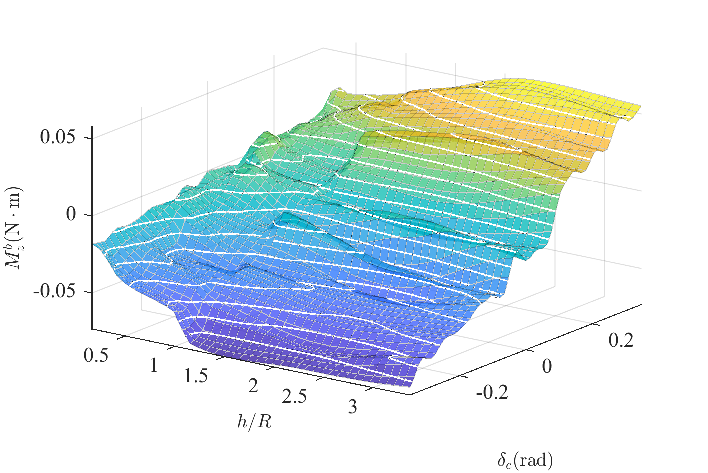
\includegraphics{matlab/ground_effect/pdf/moment/moment-h-delta.pdf}
    \caption{气动力矩$M_z^b$与高度比$h/R$以及控制舵面偏转角度$\delta_c$之间的关系}
    \label{fig:moment-h-delta}
\end{figure}

从整体趋势观察，在同一高度下，气动力矩 $M_z^b$ 与舵面偏转角 $\delta$ 呈现明显的正相关关系。气动力矩 $M_z^b$ 对舵面偏转角 $\delta$ 的斜率反映了控制舵面偏转力系数 $K_{cvGE}$ 的大小，该斜率越大，表明舵面偏转对力矩的贡献越显著。当无量纲高度 $h/R < 2.0$ 时，随着离地高度的增加，该斜率逐渐增大；当 $h/R > 2.0$ 后，无人机逐渐远离地效区，斜率趋于平缓。这一变化规律与地面效应的物理机理相符：在近地面区域，涵道出口气流受地面阻塞影响，流经舵面的气流速度和动压较低，导致舵面气动效率下降；随着高度增加，气流逐渐恢复，舵面效率随之提升，直至无地效状态下的稳定值\cite{Antonio2021, luo2023numerical}。

为深入分析力矩特性与各变量之间的依赖关系，本文从两个维度对实验数据进行剖面分析。

\begin{figure}[htbp]
    \centering
    \begin{minipage}[b]{0.45\textwidth}
        \centering
        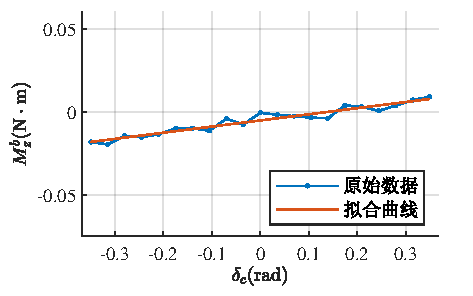
\includegraphics{matlab/ground_effect/pdf/moment/cv_moment_15mm.pdf}
        \caption*{a. $h/R = 0.17$}
    \end{minipage}
    \hfill  % 产生弹性水平间距
    \begin{minipage}[b]{0.45\textwidth}
        \centering
        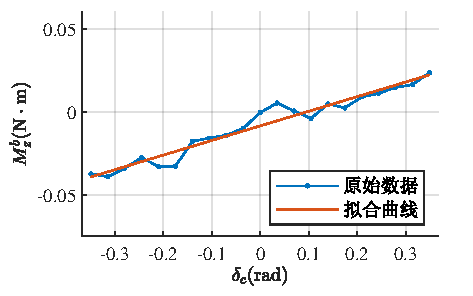
\includegraphics{matlab/ground_effect/pdf/moment/cv_moment_40mm.pdf}
        \caption*{b. $h/R = 0.45$}
    \end{minipage}

    \vspace{0.5cm}

    \centering
    \begin{minipage}[b]{0.45\textwidth}
        \centering
        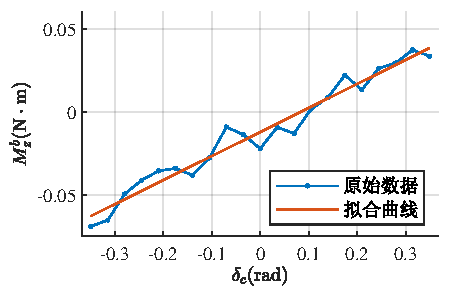
\includegraphics{matlab/ground_effect/pdf/moment/cv_moment_100mm.pdf}
        \caption*{c. $h/R = 1.12$}
    \end{minipage}
    \hfill  % 产生弹性水平间距
    \begin{minipage}[b]{0.45\textwidth}
        \centering
        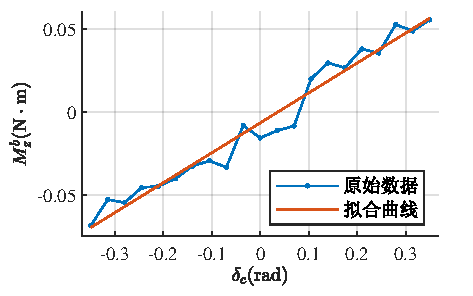
\includegraphics{matlab/ground_effect/pdf/moment/cv_moment_300mm.pdf}
        \caption*{d. $h/R = 3.36$}
    \end{minipage}
    \caption{不同高度比$h/R$下扭矩$M_z^b$与舵面角度$\delta_c$的关系}
    \label{fig:cv_moment-delta}
\end{figure}

首先，固定无量纲高度 $h/R$，考察气动力矩 $M_z^b$ 与舵面偏转角 $\delta_c$ 之间的关系。图\ref{fig:cv_moment-delta}选取了四个典型高度比 $h/R = 0.17$、$0.45$、$1.12$ 和 $3.36$ 下的实验结果。图中浅蓝色带点标记的实线为该高度下的实测力矩均值，橙色实线为通过最小二乘法拟合的线性关系线。可见，在不同高度比下，即使近地面流场相对紊乱，气动力矩 $M_z^b$ 与舵面偏转角 $\delta_c$ 之间仍呈现良好的线性关系。这一结果验证了第\ref{subsec:cv_model}节所提假设的合理性，即地面效应下舵面产生的升力与其偏转角度仍保持线性关系，地面效应主要通过衰减系数 $C_{cvGE}$ 对线性增益进行调制。此外，对比不同高度下的拟合直线可以发现，随着 $h/R$ 增大，拟合直线的斜率 $a_i$ 逐渐增大，反映出控制舵面偏转力系数 $K_{cvGE}$ 随离地高度增加而增大的趋势，这与式\eqref{eq:CcvGE_model}所描述的指数衰减规律相吻合。

\begin{figure}[htbp]
    \centering
    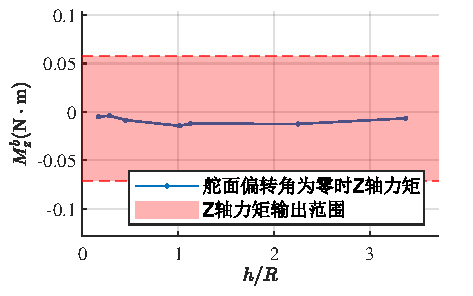
\includegraphics{matlab/ground_effect/pdf/moment/zero_output_moment.pdf}
    \caption{零输出时扭矩$M_z^b$与离地高度$h$的关系}
    \label{fig:zero_output-moment}
\end{figure}

其次，考察舵面零偏转状态下的残余力矩特性。将各高度下 $M_z^b$ 与 $\delta_c$ 线性拟合的截距 $b_i$ 作为该高度下舵面无偏转时的气动力矩 $M_{z0}^b$，并将其与无量纲高度 $h/R$ 的关系绘制于图\ref{fig:zero_output-moment}中。图中浅蓝色带点标记的实线为各高度下的实测 $M_{z0}^b$，粉红色区域表示无地面效应时（$h/R > 4.0$）的力矩输出范围。从图中可以看出，在各高度下，$M_{z0}^b$ 并非为零，这是由涵道风扇反扭矩与反扭矩襟翼产生的平衡力矩未能完全抵消所致。由于加工与装配误差，两者之间存在的残余力矩在测量中表现为恒定的偏置。进一步分析可知，$M_{z0}^b$ 随高度变化的波动幅度仅占控制舵面产生力矩变化幅度的 $7\%$ 以内，表明该残余力矩受地面效应的影响较小。因此，在后续建模中将其视为与高度无关的固定偏置量，不予纳入地面效应的动态补偿范围。

基于上述线性拟合结果，可进一步计算各高度下的控制舵面偏转力系数 $K_{cvGE}$。根据式\eqref{eq:M_cv_GE}，在四个舵面同步偏转相同角度 $\delta_c$ 的条件下，有：
\begin{equation}
    K_{cvGE} = \frac{M_z^b}{l_2(\delta_1 + \delta_2 + \delta_3 + \delta_4)} = \frac{M_z^b}{4 l_2 \delta_c},
    \label{eq:KcvGE_exp}
\end{equation}
其中 $l_2$ 为控制舵面压心到机体坐标系 $O_bZ_b$ 轴的距离，由表\ref{tab:params}给出。由于气动力矩 $M_z^b$ 与舵面偏转角 $\delta_c$ 呈线性关系，其最小二乘拟合斜率 $a_i$ 即为 $M_z^b / \delta_c$ 的估计值。因此，高度 $h_i$ 对应的控制舵面偏转力系数可近似为：
\begin{equation}
K_{cvGE,i} = \frac{a_i}{4 l_2}.
\label{eq:KcvGE_fit}
\end{equation}

\begin{figure}[htbp]
    \centering
    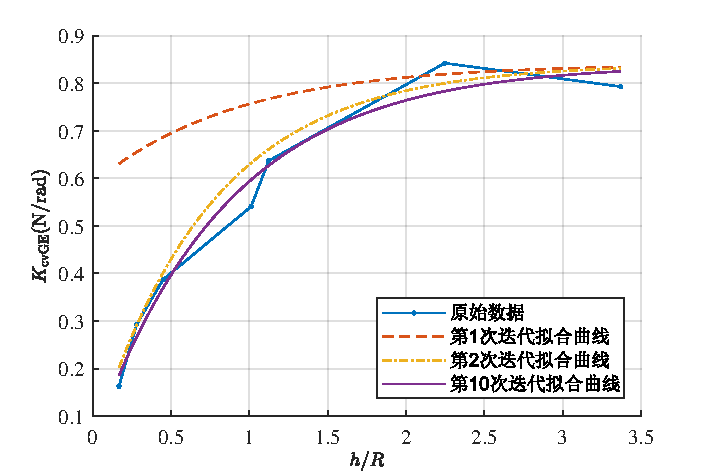
\includegraphics{matlab/ground_effect/pdf/moment/K_cv-h.pdf}
    \caption{控制舵面偏转力系数$K_{cvGE}$与高度比$h/R$的关系}
    \label{fig:K_cv-h}
\end{figure}

将各高度 $h_i$ 与其对应的 $K_{cvGE,i}$ 绘制于图\ref{fig:K_cv-h}中。从图中可以看出，$K_{cvGE,i}$ 随无量纲高度 $h/R$ 的变化呈现明显的指数增长趋势：当 $h/R < 1.5$ 时，$K_{cvGE}$ 从约 $0.2$ 迅速上升至 $0.7$；当 $1.5 < h/R < 2.0$ 时，增长速率减缓，$K_{cvGE}$ 缓慢上升至约 $0.75$；当 $h/R > 2.0$ 时，$K_{cvGE}$ 基本保持稳定，趋近于无地效状态下的基准值。这一变化规律与第\ref{subsec:cv_model}节提出的指数衰减模型式\eqref{eq:CcvGE_model}高度吻合：随着高度增加，地面效应的阻塞作用减弱，舵面气动效率逐渐恢复至无地效水平。

综合上述分析，可以得出以下结论：控制舵面产生的气动力矩与舵面偏转角在不同高度下均保持线性关系；舵面偏转力系数 $K_{cvGE}$ 随高度增加呈指数增长，在 $h/R < 1.5$ 时增长迅速，在 $h/R > 2.0$ 时趋于饱和；舵面无偏转时的残余力矩受高度影响较小，可作为固定偏置处理。这些实验数据将为第\ref{subsec:torque_fitting}节的模型参数辨识提供直接的依据。

\subsection{参数拟合}
\label{subsec:torque_fitting}
与第\ref{subsec:thrust_fitting}节推力模型的参数辨识方法类似，由于所建立的控制力矩模型为非线性形式，本节采用高斯-牛顿迭代法对衰减系数 $C_{cvAmp}$ 和 $C_{cvExp}$ 进行非线性最小二乘拟合，以确定地面效应下控制舵面偏转力系数 $K_{cvGE}$ 随高度变化的完整数学描述。

由式\eqref{eq:KcvGE}和式\eqref{eq:CcvGE_model}可知，地面效应下控制舵面偏转力系数和参数之间的关系为：
\begin{equation}
    K_{cvGE} = K_{cv}(1 - C_{cvAmp} \cdot e^{C_{cvExp} \cdot (h/R)}),
    \label{eq:KcvGE_model}
\end{equation}
其中$K_{cv}$为无地效状态下的控制舵面偏转力系数，本文实测值为$0.84\,mathrm{(N/rad)}$。
定义高度为$h_i$时的拟合误差$E_{cvGE,i}$为$K_{cvGE,i}$与模型计算值$K_{cvGE}$, $n$为拟合数据点个数：
\begin{equation}
    E_{cvGE,i} = K_{cvGE,i} - K_{cv}(1 - C_{cvAmp} \cdot e^{C_{cvExp} \cdot (h_i/R)}), \quad i = 1,2,\dots,n.
\end{equation}

参数拟合的目标是求取使误差平方和最小的参数组合，即求解如下优化问题：
\begin{equation}
    \min_{C_{cvAmp}, C_{cvExp}} \quad \sum_{i=1}^{n} E_{cvGE,i}^2.
\end{equation}
定义误差向量$\boldsymbol{E}_{cvGE} \in \mathbb{R}^{n \times 2}$为：
\begin{equation}
    \boldsymbol{E}_{cvGE} = [E_{cvGE,1}, E_{cvGE,2}, \dots, E_{cvGE,n}]^{T}.
\end{equation}
根据高斯-牛顿法，在第 $k$ 次迭代时，需计算误差向量关于参数的雅可比矩阵 $\boldsymbol{J}_{cv}^{(k)} \in \mathbb{R}^{n \times 2}$，其元素为：
\begin{equation}
    \begin{cases}
        \dfrac{\partial E_{cvGE,i}}{\partial C_{cvAmp}} = K_{cv} \, e^{C_{cvExp} (h_i/R)},\\[8pt]
        \dfrac{\partial E_{cvGE,i}}{\partial C_{cvExp}} = (h_i/R)\, K_{cv}\, C_{cvAmp} \, e^{C_{cvExp} (h_i/R)}.
    \end{cases}
    ,\quad i = 1,2,\dots,n.
\end{equation}

高斯-牛顿迭代法中的迭代步长 $\boldsymbol{\delta}_{cvGE}^{(k)} = [\Delta C_{cvAmp}, \Delta C_{cvExp}]^{T}$ 由正规方程确定：
\begin{equation}
    \boldsymbol{\delta}_{cvGE}^{(k)} = -\left( (\boldsymbol{J}_{cv}^{(k)})^{T} \boldsymbol{J}_{cv}^{(k)} \right)^{-1} (\boldsymbol{J}_{cv}^{(k)})^{T} \boldsymbol{E}_{cvGE}^{(k)}.
\end{equation}
参数更新公式为：
\begin{equation}
    \boldsymbol{\theta}_{cv}^{(k+1)} = \boldsymbol{\theta}_{cv}^{(k)} + \boldsymbol{\delta}_{cvGE}^{(k)},
\end{equation}
其中 $\boldsymbol{\theta}_{cv}^{(k)} = [C_{cvAmp}^{(k)}, C_{cvExp}^{(k)}]^{T}$。

本文选取参数初始值 $C_{cvAmp}^{(0)} = 0.3$，$C_{cvExp}^{(0)} = -1.1$，共执行 $10$ 次迭代。第$1$次，第$2$次以及第$10$次迭代的拟合结果如图\ref{fig:K_cv-h}所示。迭代过程中参数的收敛曲线如图\ref{fig:cv_param_iter}所示，误差平方和 $\sum E_{cvGE,i}^2$ 随迭代次数的变化如图\ref{fig:errr_iter}所示。

\begin{figure}[htbp]
    \centering
    \begin{minipage}[b]{0.45\textwidth}
        \centering
        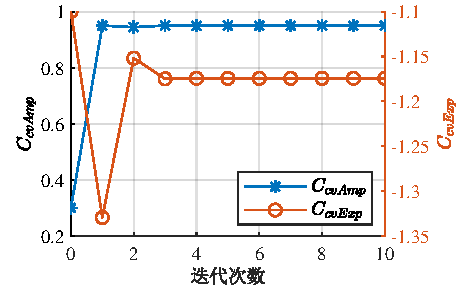
\includegraphics{matlab/ground_effect/pdf/moment/cv_param-iter.pdf}
        \caption{拟合参数与迭代次数的关系}
        \label{fig:cv_param_iter}
    \end{minipage}
    \hfill  % 产生弹性水平间距
    \begin{minipage}[b]{0.45\textwidth}
        \centering
        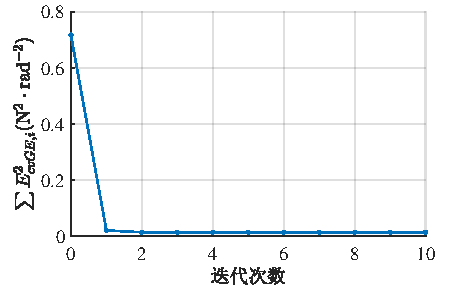
\includegraphics{matlab/ground_effect/pdf/moment/errr-iter.pdf}
        \caption{拟合误差平方和与迭代次数的关系}
        \label{fig:errr_iter}
    \end{minipage}
\end{figure}

由于该迭代算法在收敛点附近具有二次收敛速度，从图中能够看出，经过3次迭代后，拟合参数已基本趋于稳定，误差平方和迅速减小至初始值的 $1.8\%$，表明算法收敛速度较快。经过$10$次迭代，得到的参数值为：
\begin{equation}
    C_{cvAmp} = 0.950,\qquad C_{cvExp} = -1.174.
\end{equation}

将上述参数代入控制舵面偏转力系数模型\eqref{eq:KcvGE_model}，并结合$K_{cv} = 0.84\, \mathrm{N/rad}$，可给出该模型在该机型下的具体表达式：
\begin{equation}
    K_{cvGE} = 0.84\left(1 - 0.950 \cdot e^{-1.174 \cdot (h/R)}\right),
\end{equation}
其中$K_{cvGE}$单位为$\mathrm{N/rad}$。其最终拟合结果即第$10$次迭代拟合曲线已在图\ref{fig:K_cv-h}给出。从图中可以看出，拟合曲线与实验数据吻合良好，验证了所提指数衰减模型能够准确描述控制舵面偏转力系数随离地高度的变化规律。该模型将在后续章节中用于近地面抗扰控制器的设计与补偿。

\section{本章小结}

本章围绕涵道式无人机在近地面飞行时的执行器控制效益问题，系统开展了地面效应下的推力与舵面偏转力离线辨识研究。针对涵道风扇在近地面工作时推力与舵面效率发生显著变化的物理特性，分别建立了推力模型与控制舵面偏转力模型，并通过静态台架实验完成了模型参数的辨识。

首先，从地面效应的物理机理出发，分析了涵道出口射流受地面阻滞后形成高压区与反弹涡环的流场特征，阐明了推力随高度非单调变化及舵面效率降低的成因。在此基础上，采用指数衰减模型描述推力随无量纲高度 $h/R$ 的变化规律，并基于结构对称性与力矩解耦原理，建立了控制舵面偏转力系数的指数衰减模型。两类模型均满足无地效边界条件，形式简洁且物理意义明确。

其次，搭建了基于六维力/力矩传感器的变高度静态测试台架，设计了系统性的实验流程。通过调节约束板高度与螺旋桨转速，采集了不同高度下涵道风扇推力与舵面偏转力矩的稳态数据。实验结果表明，推力与转速平方在不同高度下均保持良好线性关系，控制力矩与舵面偏转角亦呈现显著线性关系，验证了模型假设的合理性。

最后，采用高斯-牛顿迭代法对模型参数进行非线性最小二乘拟合。推力模型辨识结果为 $C_{TAmp} = 0.378$、$C_{TExp} = -1.105$；控制舵面偏转力模型辨识结果为 $C_{cvAmp} = 0.950$、$C_{cvExp} = -1.174$。两者均在三步迭代内收敛，残差平方和降至初始值的 $2\%$ 以内，表明模型能够准确刻画地面效应下执行器效益随高度的变化规律。

本章所建立的推力模型与舵面偏转力模型，为后续近地面抗扰控制器设计提供了精确的执行器效益补偿依据，是提升涵道式无人机在起降、低空悬停等工况下控制性能的重要基础。